\section{Introduction}
\label{sec:intro}

Spatial transcriptomics (ST) measures expression while preserving tissue organization, but dense capture grids can repeatedly sample morphologically similar regions. This motivates testing whether fewer measured spots can supervise morphology-to-expression prediction~\cite{stahl2016visualization,zhu2024asign}. ST-Net established patch-to-spot regression~\cite{he2020integrating}; SCR$^2$-ST uses reinforcement learning for active sampling~\cite{zhu2025scr2}. Here we fix the predictor and compare standard acquisition rules. The contribution is an empirical benchmark, not a new active-learning (AL) algorithm or a demonstrated reduction in assay cost.

AL in ST differs from conventional classification: labels are multivariate continuous vectors, candidates are spatially correlated, and pointwise accuracy need not agree with spatial-pattern fidelity. Budget can also alter acquisition behavior~\cite{hacohen2022active}. We therefore compare Random with four uncertainty- or diversity-based rules over four budgets, using patient-level evaluation and three measures. The practical question is whether informed selection yields a consistent gain despite its scoring computation. A negative answer in this setting is informative, but does not establish that Random is optimal, equivalent to active selection, or sufficient for a physically realizable assay.

\begin{figure}[t]
\centering
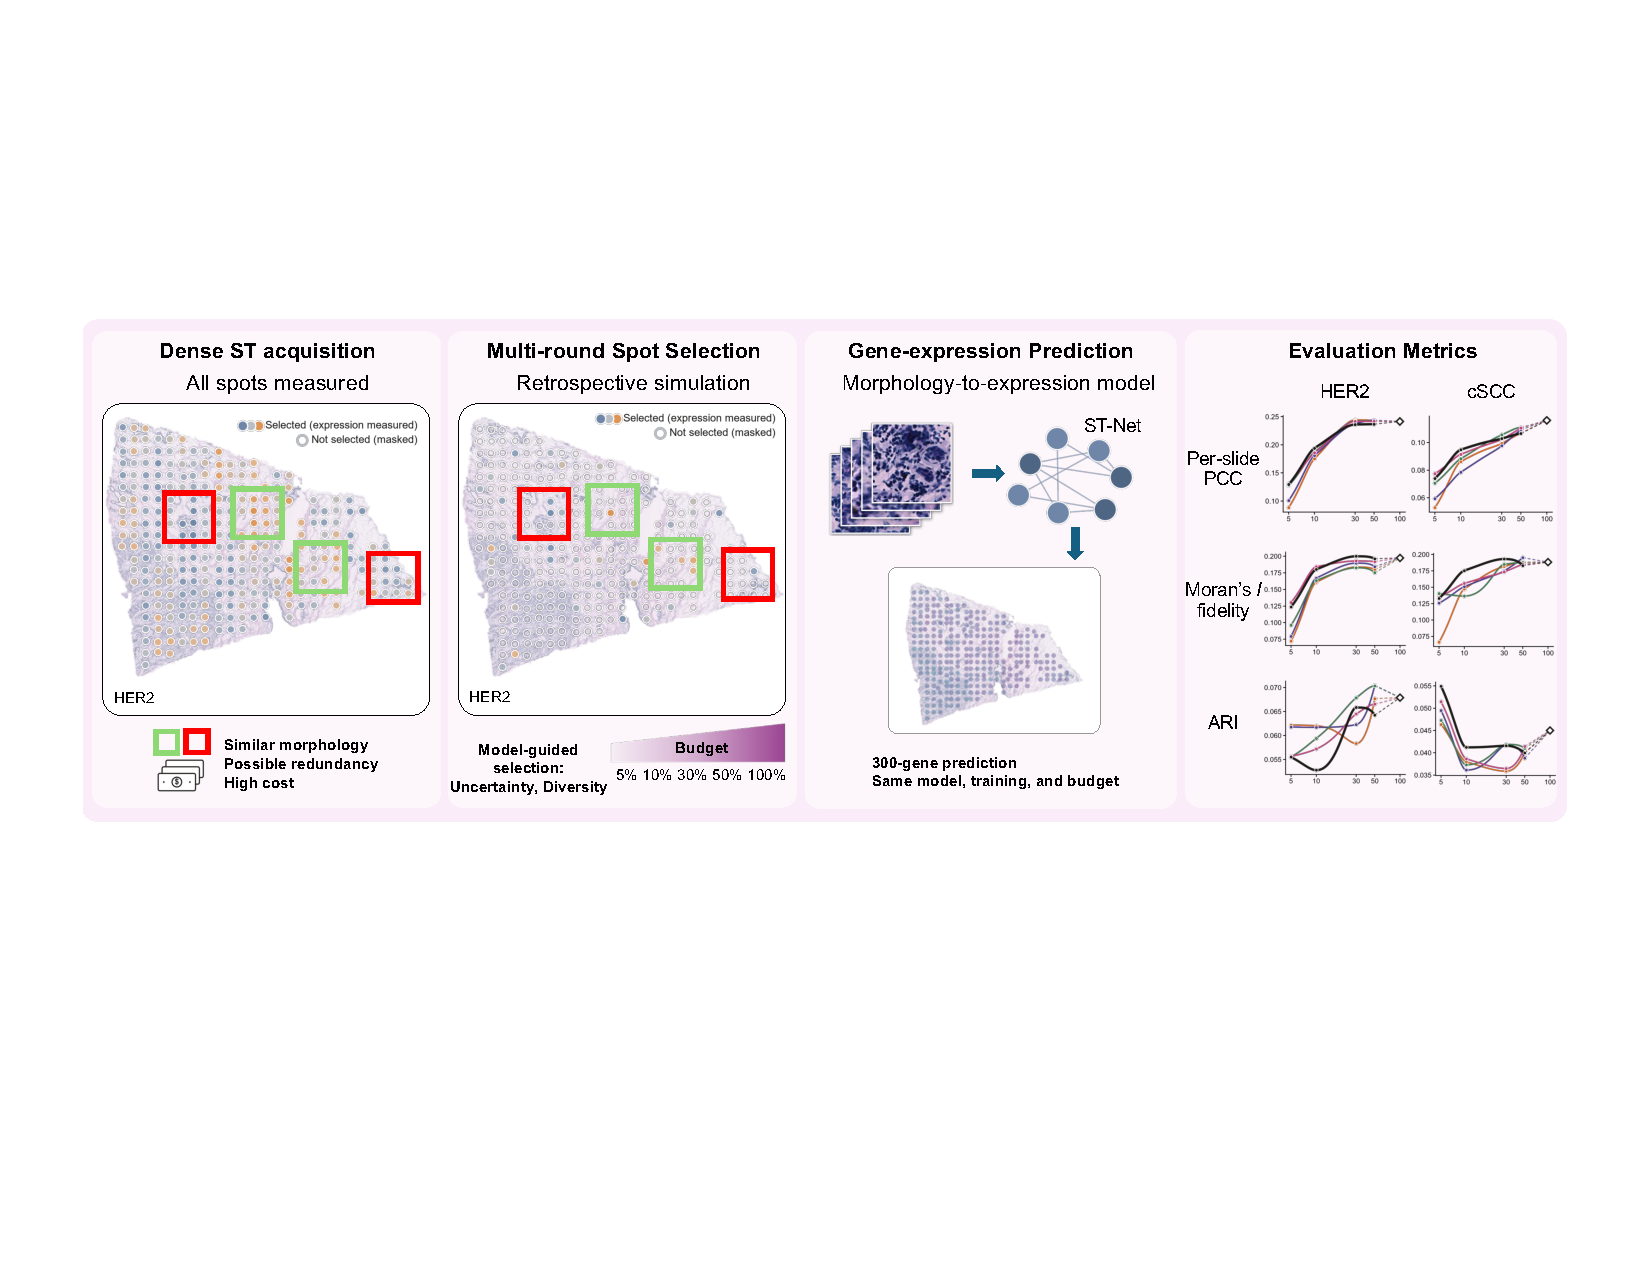
\includegraphics[width=\textwidth]{Figure/Image1.pdf}
\caption{Retrospective benchmark. All candidate H\&E images are available; only expression labels are masked. Each budget is a separate six-round training experiment. The 100\% ticks and dashed connections denote a contextual nominal full-label reference, not an optimization-matched upper bound. Outlines illustrate possible morphological redundancy. Colors: Random (black), CoreSet (orange), MC-dropout (purple), TOD (green), TypiClust-inspired (magenta).}
\label{fig:overview}
\end{figure}

\section{Methods}
\label{sec:method}
\subsection{Retrospective Active Spot-Selection Benchmark}
\label{sec:benchmark}

Starting from fully profiled cohorts, we hide expression labels in a candidate pool containing all training-fold spots across patients and slides. Selecting spot $i$ reveals its full $G=300$-gene vector; unselected expression and held-out patients remain unavailable to acquisition. The budget counts spots, not genes, images, reads, or reagent cost, and does not enforce equal slide coverage.

For $N$ candidates and budget $\beta\in\{0.05,0.10,0.30,0.50\}$, six rounds release $q=\lfloor\beta N/6\rfloor$ spots each, giving $6q$ labels. The first round is Random for every strategy. Acquisition occurs before updates at zero-indexed epochs 0, 5, 8, 11, 14, and 17 within one continuous run; the predictor is not reset. Within each budget, splits, quotas, schedules, predictor, and optimizer settings are shared across strategies, while stochastic training variation remains. The nominal full-label reference uses Random release over the same six rounds at $\beta=1$, without informed scoring, and trains for 50 epochs. Integer quotas can omit up to five spots. It is not fully labeled from epoch one or matched in optimizer exposure to lower budgets.

\subsection{Acquisition Strategies}
\label{sec:strategies}

Selection is without replacement; scoring uses deterministic preprocessing. \textbf{Random} samples uniformly over spots without a scoring pass, so expected patient/slide allocation is proportional to candidate count. \textbf{MC-dropout}~\cite{gal2016dropout} ranks candidates by predictive variance averaged across genes from five stochastic passes, enabling head dropout ($p=0.3$) while leaving batch normalization in evaluation mode. Outputs are not gene-wise standardized, so gene scale can influence this score.

\textbf{Temporal output discrepancy (TOD)}~\cite{huang2021semi} uses $\|f_{\theta_t}(x_i)-f_{\theta_{t-1}}(x_i)\|_2$, caching earlier predictions by spot identifier. Its first post-warm-up round lacks a cache and falls back to Random, leaving four informed rounds versus five for the other active rules. \textbf{CoreSet}~\cite{sener2018active} greedily selects the candidate farthest from its nearest labeled center in the unnormalized, 1,024-dimensional pooled DenseNet feature space. This is feature coverage, not physical coverage. \textbf{TypiClust-inspired}~\cite{hacohen2022active} clusters current candidate features using $k$-means ($n_{\mathrm{init}}=3$), with cluster count equal to the round quota, then selects typical members using up to 20 within-cluster neighbors. Its task-predictor features and quota-based cluster count differ from the published self-supervised implementation.

\subsection{Shared Morphology-to-Expression Predictor and Training}
\label{sec:predictor}

The ST-Net-style predictor~\cite{he2020integrating} has an ImageNet-pretrained DenseNet-121 trunk~\cite{huang2017densely} (torchvision \texttt{IMAGENET1K\_V1}), global average pooling, a 1,024-unit linear layer, ReLU, dropout, and 300 outputs. All parameters train under MSE. Training uses SGD with momentum 0.9, weight decay $10^{-4}$, batch size 80, and the final partial batch retained. At optimizer-update index $u$, the learning rate is
\begin{equation}
\eta(u)=10^{-4}(1-u/10^8)^{0.9},
\label{eq:lr}
\end{equation}
The denominator is $10^8$ updates, not the epoch horizon, so decay is nearly negligible here. Horizons are 110, 80, 70, and 60 epochs for increasing budgets, with final-checkpoint evaluation. For HER2 fold 1 ($N=9{,}810$), delivered labels are 486, 978, 2,940, and 4,902, corresponding to 715, 930, 2,260, and 3,156 updates. Cross-budget comparisons therefore do not match exposure or convergence.

Augmentation applies independent horizontal/vertical flips ($p=0.5$ each), then a $90^\circ$ rotation ($p=0.5$); there is no stain normalization or color augmentation. Every configuration uses seed 42 on one RTX 3080 (10~GB), with Python 3.11.15, PyTorch 2.6.0, torchvision 0.21.0, CUDA 12.4, cuDNN 9.1.0, and scikit-learn 1.9.0. Deterministic algorithms are disabled and training noise is not paired across strategies.

\section{Data and Experimental Design}
\label{sec:data}
\subsection{Datasets and Targets}
\label{sec:setup}

The public HEST-1k~\cite{jaume2024hest} cohorts are HER2-positive breast cancer~\cite{andersson2021spatial} and cSCC~\cite{ji2020multimodal} (Table~\ref{tab:datasets}). Four-fold patient-level cross-validation holds out two HER2 patients per fold (nine slides; 2,457--3,810 spots), or one cSCC patient (three slides; 1,632--3,398 spots). Five strategies, four budgets, and four folds give 160 completed budgeted configurations; eight nominal full-label references are separate. Each configuration, including Random, has one training/acquisition seed.

\begin{table}[htbp]
\centering
\caption{Cohort size, H\&E scale, and physical context of 224-pixel patches. Image scale is distinct from ST capture-spot resolution.}
\label{tab:datasets}
\begin{tabular}{lrrrrr}
\hline
Cohort & Patients & Slides & Spots & $\mu$m/pixel & Patch width ($\mu$m) \\
\hline
HER2 & 8 & 36 & 13,620 & 0.662--0.946 & 148.3--212.0 \\
cSCC & 4 & 12 & 8,671 & 0.545--0.554 & 122.2--124.1 \\
\hline
\end{tabular}
\end{table}

The trainer consumes supplied \texttt{expression\_norm} vectors without further normalization, taking the first 300 alphabetically ordered retained genes. A numerical audit of row and gene correspondence against raw HEST counts $c_{ig}$ found
\begin{equation}
\tilde y_{ig}=\begin{cases}
\log(1+c_{ig}), &\text{HER2},\\
\log(1+10^4c_{ig}/L_i), &\text{cSCC},
\end{cases}
\quad L_i=\sum_{h\in\mathcal J}c_{ih}.
\label{eq:targets}
\end{equation}
Here $\mathcal J$ is the 13,251-gene intersection across the 12 raw cSCC slides, not its 392 retained genes or 300 outputs. This empirically reconstructed cSCC formula matches all $8{,}671\times300$ targets within $2.4\times10^{-7}$; HER2 raw-log targets match exactly. Random-50\% saved ground truth matches the supplied vectors on all 48 slides. The original target-producing script was not recovered. Neither panel is gene-wise standardized; cohort-specific preprocessing limits cross-cohort interpretation.

\subsection{Image Resolution and Physical Context}
\label{sec:resolution}

All 22,291 training PNG headers are $224\times224$, but patch width in micrometers is $224$ times slide scale (Table~\ref{tab:datasets}). Twelve sampled patches from four available HER2 whole-slide images match native-resolution crops exactly. cSCC scale relies on corresponding metadata because its whole-slide images were unavailable locally. Training PNGs differ from HEST's separately downsampled HDF5 patch product. Resizing an already 224-pixel patch does not harmonize physical context. Paired strategies receive identical images and scales; this controls an input difference between arms, not invariance to scale. Patient and acquisition characteristics remain confounded; no common-field-of-view retraining or multiple-capture-resolution experiment was performed.

\subsection{Evaluation and Reporting}
\label{sec:evaluation}

\textbf{PCC} is computed across spots for each gene within a held-out slide, averaged over genes and then equally over slides within the fold. Correlations are averaged directly, without Fisher transformation; a $10^{-8}$ denominator stabilizer makes constant genes contribute approximately zero. \textbf{Expression-cluster agreement} independently clusters measured and predicted profiles within each slide ($k$-means, $k=10$, $n_{\mathrm{init}}=10$, seed 42; no scaling/PCA), then computes ARI~\cite{hubert1985comparing}; slides with fewer than $2k$ spots are excluded. This is not histological-domain recovery. \textbf{Moran's $I$ fidelity}~\cite{moran1950notes} correlates measured and predicted gene-wise $I$ across at least three defined genes, using a symmetrized six-nearest-neighbor graph on array coordinates with binary, non-row-standardized weights. Spatial measures are averaged over evaluable slides, then equally over folds.

\textbf{Statistical reporting.} The comparison unit is a paired fold, not a spot or gene. We report means, sample SDs, paired active-minus-Random effects, and fold signs. Four strategies sharing Random do not supply 16 independent observations; fold SD does not estimate seed variability. As an exploratory sensitivity analysis, the corrected CV statistic~\cite{bouckaert2004replicability} uses $\mathrm{SE}_{\mathrm{corr}}=\sqrt{(1/4+1/3)s_d^2}$ for four differences with sample variance $s_d^2$, $t=\bar d/\mathrm{SE}_{\mathrm{corr}}$, and three degrees of freedom. The nominal held-out/training patient ratio is $1/3$. Holm adjustment~\cite{holm1979simple} covers all 32 PCC comparisons, with two-sided $\alpha=0.05$; approximate 95\% intervals are pointwise. This heuristic is not calibrated for four heterogeneous grouped-regression folds and cannot measure seed variability or establish equivalence. Spatial metrics and pooled/reference summaries remain descriptive.

\section{Results}
\label{sec:results}
\subsection{Gene-Expression Accuracy and Training Horizons}

PCC generally rises with budget, while between-fold variation exceeds mean differences among strategies (Table~\ref{tab:pcc}). After 50 epochs, nominal full-label reference means are $0.2416\pm0.1460$ on HER2 and $0.1160\pm0.0220$ on cSCC. To quantify horizon sensitivity, define $r=100(\bar p_E-\bar p_{E-10})/\bar p_E$ from four-fold mean PCC. Across strategies/cohorts, final-ten-epoch changes range from $+10.1$\% to $+27.8$\% at 5\%, $+4.6$\% to $+23.0$\% at 10\%, $-3.3$\% to $+3.5$\% at 30\%, and $-2.0$\% to $+4.0$\% at 50\%. These are horizon-dependent results, not convergence guarantees.

%%PCC_TABLE%%

At common epoch 50, nominal full-label minus Random-50\% is $+0.0058$ on HER2 (3/4 positive folds) and $+0.0073$ on cSCC (4/4). The reference receives 5,028--5,721 and 2,695--3,600 optimizer updates, respectively, versus 2,536--2,865 and 1,353--1,804 for the half-budget arm. This checks elapsed-epoch sensitivity without matching updates or labeled-example presentations; it is not an optimization-matched upper bound.

\subsection{Paired Comparison With Random}

Three of four active means are below Random at 5\% and all four at 10\% on both cohorts (Table~\ref{tab:paired}). At 30\%, all four differences are positive on HER2 but three remain negative on cSCC; all four are slightly positive at 50\% on both cohorts. There is no shared 30\% crossover. None of the 32 exploratory corrected tests reaches $0.05$ before or after Holm adjustment (minimum unadjusted $p=0.128$; all adjusted $p=1.000$). HER2 CoreSet at 5\% has $\bar d=-0.0412$, 0/4 positive folds, and approximate corrected 95\% interval $[-0.1041,0.0216]$. Non-rejection does not establish zero effect or equivalence. Complete paired values and sensitivity outputs are retained in the revision's validation materials.

%%POOLED_TABLE%%

\subsection{Spatial-Expression Structure}

At 5\%/10\% on HER2, CoreSet and MC-dropout have lower mean PCC but higher ARI than Random, with ARI positive on every fold; lower PCC is not universal across folds. Every active mean ARI is below Random on cSCC at those budgets (Table~\ref{tab:spatial}). This dissociation therefore does not reproduce across cohorts. TypiClust-inspired has the highest HER2 mean Moran fidelity at 5\%/10\%, while Random leads at 30\%/50\% (0.1999/0.1962); the cSCC leader varies. Low absolute agreement and metric-dependent rankings argue for separate outcomes, not interchangeable measures of biological success. Figure~\ref{fig:predmaps} illustrates one held-out slide without ranking strategies; all-budget spatial summaries are provided in the validation materials.

%%SPATIAL_TABLE%%

\begin{figure}[htbp]
\centering
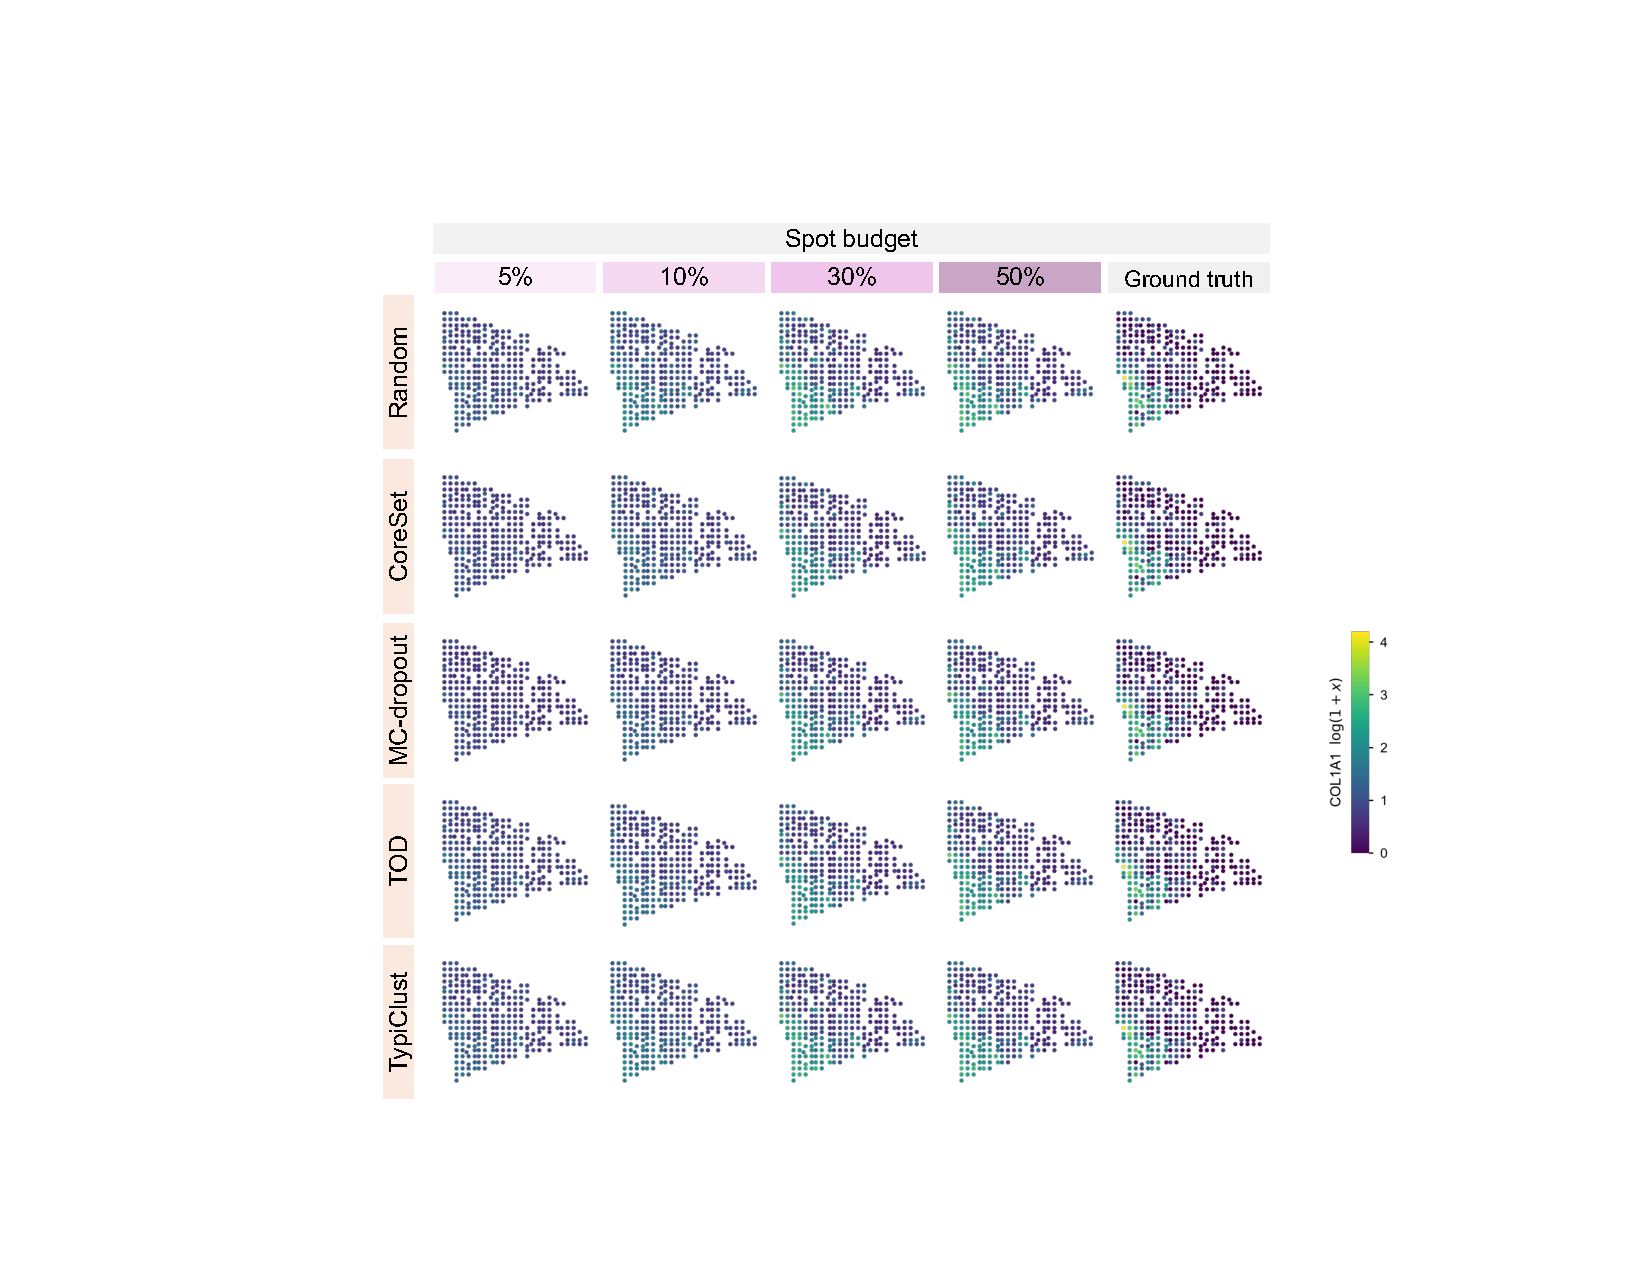
\includegraphics[width=0.80\textwidth]{Figure/Image2.pdf}
\caption{Predicted \textit{COL1A1} on held-out HER2 slide SPA143. Rows are strategies and columns are budgets; every panel shares the measured-map scale. Predicted SD rises from 0.18--0.28 at 5\% to 0.67--0.70 at 50\%, versus 0.87 measured. This single-slide illustration is not used to rank methods.}
\label{fig:predmaps}
\end{figure}

\section{Discussion and Future Work}
\label{sec:discussion}
\subsection{What the Negative Result Establishes}

These implementations provide no consistent low-budget PCC gain over Random under the reported protocol, despite additional scoring computation. This bounded negative finding answers the benchmark question without establishing universal AL failure or statistical equivalence. Thousands of spots do not replace independent patients: generalization is evaluated on only eight HER2 and four cSCC patients. The higher-budget direction is cohort-specific, and the PCC/ARI reversal is also cohort-specific. Neither implies a universal budget threshold or biological-domain recovery.

Scoring times include feature extraction but exclude training. At HER2 50\%, ranges of within-fold median logged scoring times are 10.7--12.3 seconds for CoreSet, 37.1--41.8 for MC-dropout, and 7.4--8.4 for TOD. Three later-session TypiClust-inspired fold medians range from 71.1--83.1 seconds, versus an earlier 1,584.3-second median. Sessions differ in date and quota; no monitored-load repetitions establish the cause. These are implementation-specific logs, not controlled timing or assay-cost measurements.

\subsection{Uncertainty and Experimental Controls}

One acquisition/training seed per configuration leaves acquisition randomness, optimization randomness, their interaction, and CUDA nondeterminism inseparable. Four overlapping folds measure held-out-patient heterogeneity, not repeated-seed reproducibility. The exploratory correction cannot replace repeated independent seeds, multiple Random realizations, repeated patient partitions where feasible, and dependence-aware uncertainty analysis. Equivalence/noninferiority would require a justified practical margin and adequate power. Small-budget models remain horizon-sensitive; convergence-controlled and optimizer-step-controlled comparisons are future controls.

\subsection{Resolution, Targets, and Generality}

Resolution was audited rather than harmonized experimentally. Future controls should independently vary H\&E micrometers/pixel, physical field of view, and capture-spot/bin geometry, matching patient/scanner where possible. Current results do not transfer automatically to higher-resolution platforms. Cohort-specific target normalization also confounds cross-cohort interpretation; scale affects MSE and uncertainty/discrepancy scores. Normalization and gene-standardization comparisons should hold genes, splits, and predictors fixed, fitting any learned preprocessing only on training patients. Alphabetical panels warrant comparison with training-derived variable genes and biological panels.

Additional organs, including renal tissue, independent databases, platforms, and predictors are needed to test generality. Selected regions were not analyzed in these conference runs; preference for unusual morphology, boundaries, or artifacts remains hypothetical. Patient/slide allocation, dispersion, and representativeness should be measured, with patient-balanced Random and spatial baselines separating allocation from model-based scoring. TOD's extra Random round and the TypiClust adaptation also require matched controls.

\subsection{From Label Budgets to Real Acquisition}

Retrospective masking retains all images after complete profiling; it proves neither reduced image acquisition nor prospective sequencing savings. Arbitrary disconnected spots may not translate into feasible capture regions. Future assays should test contiguous masks, region/read costs, marker/pathway and rare-region preservation, expert-informed acquisition, and prospective feasibility. Until those tests exist, the reported spot fractions are supervision budgets, not demonstrated biological or economic equivalence to dense acquisition.

\section{Conclusion}

In this two-cohort, one-predictor benchmark, the tested active rules show no consistent low-budget PCC improvement over Random: three of four means are lower at 5\% and all four at 10\% on both cohorts. Larger-budget gains and metric rankings are cohort-dependent. Exploratory testing establishes neither a significant difference nor equivalence. Conclusions remain conditional on image scale, cohort-specific preprocessing, single seeds, and fixed horizons. Repeated seeds, harmonized scale/target controls, broader tissue/database validation, and physically feasible acquisition are necessary before recommending an active rule or claiming assay-cost savings.

\section*{ACKNOWLEDGMENTS}
This research was supported by the WCM Radiology AIMI Fellowship and WCM CTSC 2027 Pilot Award. Additional support was provided by NIH 1R01HL174863-01A1 (Sabuncu) and NIH 1U54DK144866-01 (Sabuncu).

\bibliography{main}
\bibliographystyle{spiebib}
\end{document}
